% Este arquivo .tex será incluído no arquivo .tex principal. Não é preciso
% declarar nenhum cabeçalho

\section{Melhores banheiros}

Uma das maiores necessidades do ser humano pode ser potencializada se for
realizada num banheiro decente. Portanto, é muito importante que você saiba onde
ir. Alguns dos melhores banheiros da Unicamp são:

\begin{itemize}
    \item  \textbf{IC-3:} Geralmente estão limpos e utilizáveis. Mas fedem. E em 
        dia de chuva ficam imundos. Sempre com papel higiênico, é uma boa pedida 
        na hora do apuro. Exceto nos finais de semana.

    \item  \textbf{IC-2:} Quase sempre estão limpos e utilizáveis e tem um odor
        melhor que os do IC-3. Só precisa tomar cuidado pois às vezes falta
        papel higiênico.

    \item  \textbf{FEEC:} Possui excelentes banheiros escondidos por lá,
        principalmente após as reformas de 2013. Procure bem!

    \item  \textbf{PB:} Os banheiros do segundo e do terceiro andar do Pavilhão
        Básico também são bons (especialmente os do terceiro andar, por quase
        não serem usados). Só tome cuidado, porque às vezes não tem papel
        higiênico.

        \begin{figure}[h!]
            \centering
            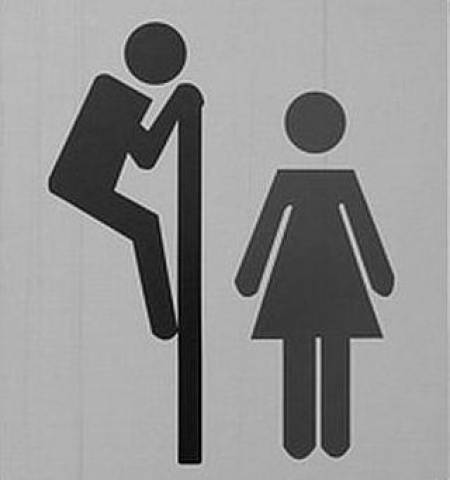
\includegraphics[scale=0.50, keepaspectratio=true]{img/imgs/12-melhores_banheiros/banheiro.jpg}
        \end{figure}

    \item  \textbf{FE:} A Faculdade de Educação tem poucos banheiros masculinos,
        mas estão entre os melhores da Unicamp pelo pouco uso.

    \item  \textbf{CB:} Estes banheiros ficam escondidos próximo às escadas do
        CB (no térreo). Se você tiver sorte de chegar bem após a limpeza, o
        banheiro estará em excelentes condições. Porém, na maior parte do tempo
        ele fica bem sujinho.

    \item  \textbf{DEQ:} Departamento de Eletrônica Quântica, no IFGW. Dizem que
        ninguém os usa.

    \item  \textbf{DRCC:} Departamento de Raios Cósmicos e Cronologia, no IFGW.
        Um dos melhores banheiros existentes na Unicamp (senão o melhor). Assim
        como os banheiros do DEQ, dizem que ninguém os usa.

    \item  \textbf{DFA:} Departamento de Física Aplicada, no IFGW. Os dois
        andares do departamento tem banheiros bons e utilizáveis, mas algumas
        vezes falta papel higiênico.

    \item  \textbf{IMECC:} Todos os três departamentos (andares) do IMECC tem
        banheiros bons e utilizáveis. Mas vez ou outra falta papel higiênico.
\end{itemize}
